\documentclass[12pt]{report}
\usepackage[utf8]{inputenc}
\usepackage[russian]{babel}
%\usepackage[14pt]{extsizes}
\usepackage{listings}
\usepackage{GOST}

\usepackage{graphicx}
\usepackage{graphicx}
\usepackage{amsmath,amsfonts,amssymb,amsthm,mathtools} 
\usepackage{float}
\DeclareGraphicsExtensions{.pdf,.png,.jpg}

\usepackage{color}
\definecolor{codegreen}{rgb}{0,0.6,0}
\definecolor{codegray}{rgb}{0.5,0.5,0.5}
\definecolor{codepurple}{rgb}{0.58,0,0.82}
\definecolor{backcolour}{rgb}{1,1,1}

% Для листинга кода:
\lstset{ %
	language=c++,                 % выбор языка для подсветки
	backgroundcolor=\color{backcolour},   
	commentstyle=\color{codegreen},
	keywordstyle=\color{magenta},
	numberstyle=\tiny\color{codegray},
	stringstyle=\color{codepurple},
	basicstyle=\small\sffamily, % размер и начертание шрифта для подсветки кода
	numbers=left,               % где поставить нумерацию строк (слева\справа)
	numberstyle=\tiny,           % размер шрифта для номеров строк
	stepnumber=1,                   % размер шага между двумя номерами строк
	numbersep=7pt,                % как далеко отстоят номера строк от подсвечиваемого кода
	showspaces=false,            % показывать или нет пробелы специальными отступами
	showstringspaces=false,      % показывать или нет пробелы в строках
	showtabs=false,             % показывать или нет табуляцию в строках
	frame=single,              % рисовать рамку вокруг кода
	tabsize=4,                 % размер табуляции по умолчанию равен 2 пробелам
	captionpos=t,              % позиция заголовка вверху [t] или внизу [b] 
	breaklines=true,           % автоматически переносить строки (да\нет)
	breakatwhitespace=false, % переносить строки только если есть пробел
	escapeinside={\#*}{*)},   % если нужно добавить комментарии в коде
}

% Для измененных титулов глав:
\usepackage{titlesec, blindtext, color} % подключаем нужные пакеты
\definecolor{gray75}{gray}{0.75} % определяем цвет
\newcommand{\hsp}{\hspace{20pt}} % длина линии в 20pt
% titleformat определяет стиль
\titleformat{\chapter}[hang]{\Huge\bfseries}{\thechapter\hsp\textcolor{gray75}{|}\hsp}{0pt}{\Huge\bfseries}


% plot
\usepackage{pgfplots}
\usepackage{filecontents}
\usetikzlibrary{datavisualization}
\usetikzlibrary{datavisualization.formats.functions}


\begin{document}
	%\def\chaptername{} % убирает "Глава"
\begin{titlepage}
	\begin{table}[ht]
		\centering
		\begin{tabular}{|c|p{400pt}|} 
			\hline
			\begin{tabular}[c]{@{}c@{}} 
\includegraphics[scale=1]{pics/b_logo.jpg} \\\end{tabular} &
			\footnotesize\begin{tabular}[c]{@{}c@{}}\textbf{Министерство~науки~и~высшего~образования~Российской~Федерации}\\\textbf{Федеральное~государственное~бюджетное~образовательное~учреждение}\\\textbf{~высшего~образования}\\\textbf{«Московский~государственный~технический~университет}\\\textbf{имени~Н.Э.~Баумана}\\\textbf{(национальный~исследовательский~университет)»}\\\textbf{(МГТУ~им.~Н.Э.~Баумана)}\\\end{tabular}  \\
			\hline
		\end{tabular}
	\end{table}
\noindent\rule{\textwidth}{4pt}
\noindent\rule[14pt]{\textwidth}{1pt}
\hfill 
\noindent
\makebox{ФАКУЛЬТЕТ~}%
\makebox[\textwidth][l]{\underline{~«Информатика и системы управления»~~~~~~~~~~~~~~~~~~~~~~~~~~~~~~~~~}}%
\\
\noindent
\makebox{КАФЕДРА~}%
\makebox[\textwidth][l]{\underline{~«Программное обеспечение ЭВМ и информационные технологии»~}}%
\\

\begin{center}
	\vspace{1.5cm}
	{\bf\huge Отчёт\par}
	{\bf\Large по лабораторной работе № 5\par}
	\vspace{0.7cm}
\end{center}


\noindent
\makebox{\large{\bf Название:}~~~}
\makebox[\textwidth][l]{\large\underline{~Конвейер~~~~~~~~~~~~~}}\\

\noindent
\makebox{\large{\bf Дисциплина:}~~~}
\makebox[\textwidth][l]{\large\underline{~Анализ алгоритмов~~~~~~~~~~~~~~~~~~~~~~~~~~}}\\

\vspace{1.5cm}
\noindent
\begin{tabular}{l c c c c c}
	Студент      & ~ИУ7-54Б~               & \hspace{3.5cm} & \hspace{2cm}                 & &  Д.Ю. Расколотов \\\cline{2-2}\cline{4-4} \cline{6-6} 
	\hspace{3cm} & {\footnotesize(Группа)} &                & {\footnotesize(Подпись, дата)} & & {\footnotesize(И.О. Фамилия)}
\end{tabular}

\noindent
\begin{tabular}{l c c c c}
	Преподователь & \hspace{6cm}   & \hspace{2cm}                 & & Л.Л. Волкова\\\cline{3-3} \cline{5-5} 
	\hspace{3cm}  &                & {\footnotesize(Подпись, дата)} & & {\footnotesize(И.О. Фамилия)}
\end{tabular}

\vspace{0.6cm}
\begin{center}	
	\vfill
	\large \textit {Москва, 2020}
\end{center}

\thispagestyle {empty}
\pagebreak
\end{titlepage}

\tableofcontents

\newpage
\chapter*{Введение}
\addcontentsline{toc}{chapter}{Введение}
Цель работы: получить навык организации конвейерных вычислений в параллельном режиме.
\begin{flushleft}
\textbf{Задачи данной лабораторной работы:}
\begin{enumerate}
	\item спроектировать ПО, реализующего конвейерную обработку;
	\item описать реализацию ПО;
	\item провести тестирование ПО.
\end{enumerate}
\end{flushleft}


\chapter{Аналитическая часть}
В данной части будут рассмотрены главные принципы конвейерной обработки и параллельных вычислений.

\section{Общие сведения о конвейерной обработке}
\par
\textbf{Конвейер} – машина непрерывного транспорта, предназначенная для перемещения сыпучих, кусковых или штучных грузов \cite{mednov}.


\textbf{Конвейерное производство} - система поточной организации производства на основе конвейера, при которой оно разделено на простейшие короткие операции, а перемещение деталей осуществляется автоматически. Это такая организация выполнения операций над объектами, при которой весь процесс воздействия разделяется на последовательность стадий с целью повышения производительности путём одновременного независимого выполнения операций над несколькими объектами, проходящими различные стадии.

\begin{flushleft}
\textbf{Каждое звено конвейера выполняет следующие действия:}
\begin{enumerate}
	\item Получить данные,
	\item Обработать данные,
	\item Послать данные следующим звеньям.

\end{enumerate}
\end{flushleft}
\section{Параллельное программирование}

При использовании многопроцессорных вычислительных систем с общей памятью обычно предполагается, что имеющиеся в составе системы процессоры обладают равной производительностью, являются равноправными при доступе к общей памяти, и время доступа к памяти является одинаковым (при одновременном доступе нескольких процессоров к одному и тому же элементу памяти очередность и синхронизация доступа обеспечивается на аппаратном уровне). Многопроцессорные системы подобного типа обычно именуются симметричными мультипроцессорами (symmetric multiprocessors, SMP).

Перечисленному выше набору предположений удовлетворяют также активно развиваемые в последнее время многоядерные процессоры, в которых каждое ядро представляет практически независимо функциони рующее вычислительное устройство.

Обычный подход при организации вычислений для многопроцессорных вычислительных систем с общей памятью – создание новых параллельных методов на основе обычных последовательных программ, в которых или автоматически компилятором, или непосредственно программистом выделяются участки независимых друг от друга вычислений. Возможности автоматического анализа программ для порождения параллельных вычислений достаточно ограничены, и второй подход является преобладающим. При этом для разработки параллельных программ могут применяться как новые алгоритмические языки, ориентированные на параллельное программирование, так и уже имеющиеся языки, расширенные некоторым набором операторов для параллельных вычислений.


\subsection{Организация взаимодействия параллельных потоков}
Потоки исполняются в общем адресном пространстве параллельной программы. Как результат, взаимодействие параллельных потоков можно организовать через использование общих данных, являющихся доступными для всех потоков. Наиболее простая ситуация состоит в использовании общих данных только для чтения. В случае же, когда общие данные могут изменяться несколькими потоками, необходимы специальные усилия для организации правильного взаимодействия.

\section{Вывод}
В данном разделе были рассмотрены основы конвейерной обработки, технология параллельного программирования и
организация взаимодействия параллельных потоков.

\chapter{Конструкторская часть}
\textbf{Требования к вводу:}
На вход в очередь №1 подаются задачи из генератора задач.
\newline
\textbf{Требования к программе при параллельной обработке:}
\begin{itemize}
	\item объекты должны последовательно проходить конвейеры в заданном подядке;
	\item конвейеры должны работать каждый в своем потоке;
	\item конвейер должен завершать свою работу при выполнении всех задач;
	\item до завершения работы конвейер должен ожидать поступления новых элементов.
\end{itemize}

\section{Организация обработки}
У каждой линии конвейера есть очередь элементов. Когда линия еще активна, но элементов в очереди нет, линия уходит в режим ожидания.
По прошествию заданного времени линия проверяет не появились ли новые элементы в очереди. Если очередь не пустая, то нужно получить и обработать элемент, передать его следующей линии, если такая существует.
\begin{center}
	На рисунке {2.1} представлена подробная схема организации конвейерной обработки.
\end{center}


\begin{figure}[pt]
	\centering
	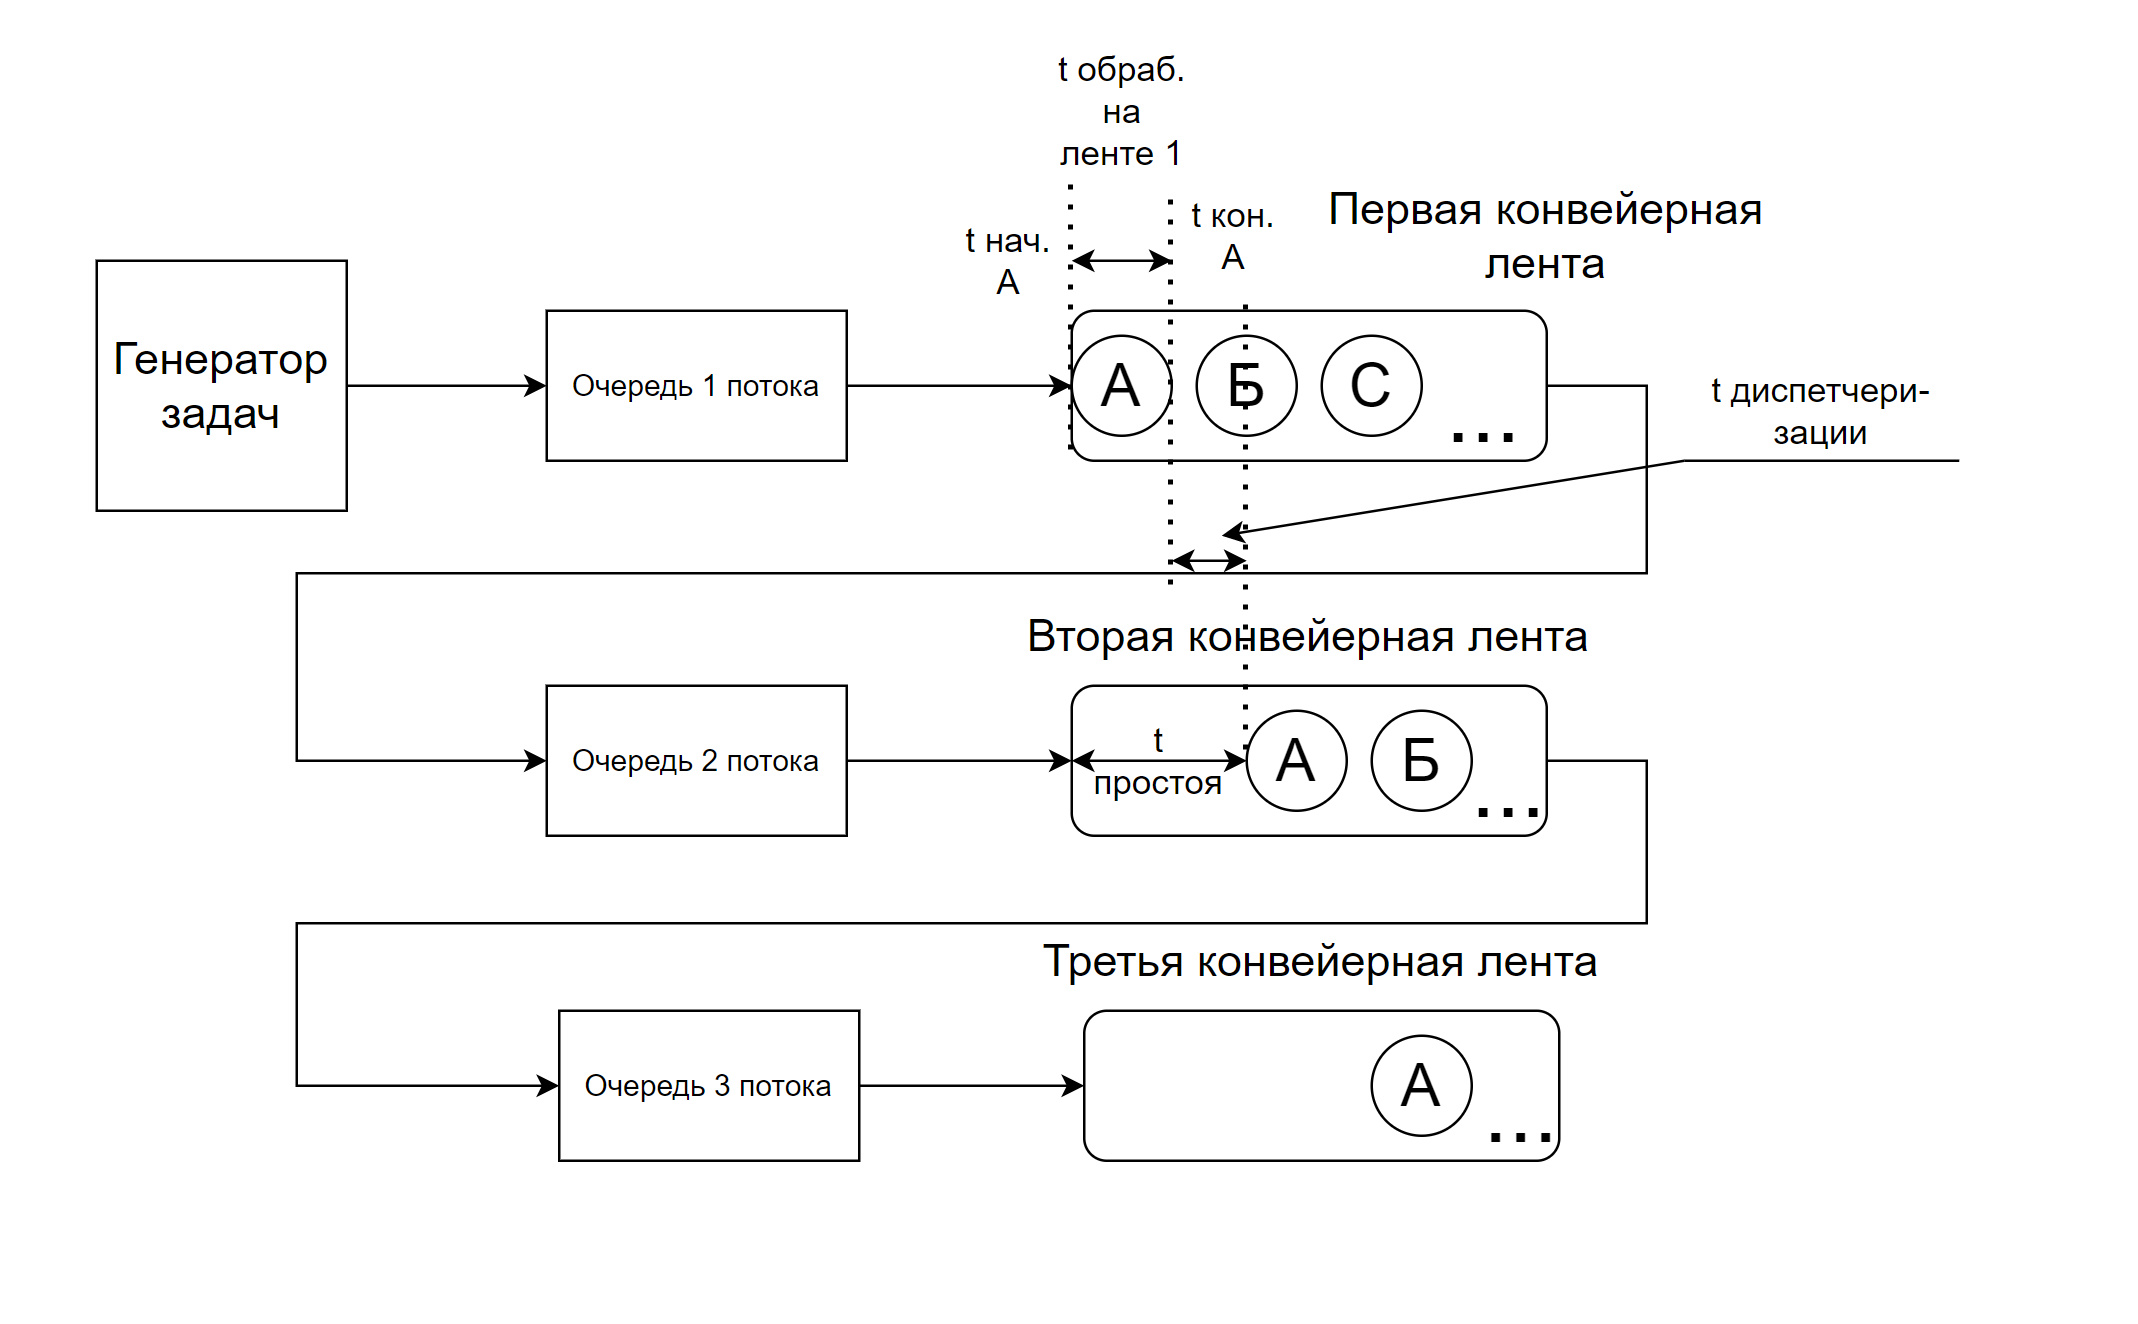
\includegraphics[height = 12cm,height=11cm]{Conveyr.jpg}
	\caption{Схема конвейерной обработки}
	\label{fig:mpr}
\end{figure}
\newpage

\section{Генератор задач}
В качестве задач, реализуемых на конвейере, я решил выбрать - сортировки. Данные, которые они будут сортировать - неизменны. То есть на вход каждой сортировки будет подаваться неотсортированный константный массив состоящий из 10000 элементов. Выбор сортировок осуществлялся, исходя из практически идентичного времени работы каждой сортировки.
\newline
\\
\textbf{Выбранные алгоритмы сортировок:}
\begin{itemize}
	\item cортировка Шейкером;
	\item cортировка Пузырьком;
	\item cортировка Пузырьком с флагом;
	\item cортировка прямыми включениями;
	\item cортировка прямым выбором.
\end{itemize}

\section{Вывод}
В данном разделе была рассмотрена схема организации конвейерной обработки. А так же выбраны соразмерные задачи для реализации конвейерной ленты.


\chapter{Технологическая часть}
Замеры времени были произведены на: Intel(R) Core(TM) i7-10510U, 4 ядра, 8 логических процессоров.

\section{Выбор ЯП}
В качестве языка программирования был выбран С++, так как этот
язык поддерживает управление потоками на уровне ОС(незеленые потоки). Средой разработки Visual Studio Code. 
Время работы алгоритмов было замерено с помощью класса <windows.h>. Многопоточное программирование было
реализовано с помощью класса Thread.

\newpage
\section{Листинг программы}
\begin{lstlisting}[label=some-code,caption= Структура объекта]
		typedef struct Log
		{
			int tape;
			int sort;
			char status;
			SYSTEMTIME time;
		} Log;
\end{lstlisting}
\par
\begin{lstlisting}[label=some-code,caption=Основная функция]
	void MainFunc()
	{
		generate_massive(a, b, c, len_mas);
		
		for (auto i = 0; i < 5; ++i)
		que1.push((i + 1));
		
		Thread threads;
		threads.push_back(thread(way1));
		threads.push_back(thread(way2));
		threads.push_back(thread(way3));
		
		for (auto &th : threads)
		th.join();
	}
\end{lstlisting}
\par
\begin{lstlisting}[label=some-code,caption=Лента №1]
	void way1()
	{
		while (true)
		{
			if (!que1.empty())
			{
				int sortN = que1.front();
				
				m.lock();
				GetSystemTime(&t);
				res.push_back({1, sortN, 'S', t});
				m.unlock();
				
				CurrentSort(sortN, a, len_mas);
				
				que1.pop();
				
				m.lock();
				GetSystemTime(&t);
				res.push_back({1, sortN, 'F', t});
				m.unlock();
				
				que2.push(sortN);
				
				if (sortN == 5)
				return;
			}
		}
	}
\end{lstlisting}
\par
\begin{lstlisting}[label=some-code,caption=Лента №2]
	void way2()
	{
		while (true)
		{
			if (!que2.empty())
			{
				int sortN = que2.front();
				
				m.lock();
				GetSystemTime(&t);
				res.push_back({2, sortN, 'S', t});
				m.unlock();
				
				CurrentSort(sortN, b, len_mas);
				
				que2.pop();
				
				m.lock();
				GetSystemTime(&t);
				res.push_back({2, sortN, 'F', t});
				m.unlock();
				
				que3.push(sortN);
				
				if (sortN == 5)
				return;
			}
		}
	}
\end{lstlisting}
\par
\begin{lstlisting}[label=some-code,caption=Лента №3]
	void way3()
	{
		while (true)
		{
			if (!que3.empty())
			{
				int sortN = que3.front();
				
				m.lock();
				GetSystemTime(&t);
				res.push_back({3, sortN, 'S', t});
				m.unlock();
				
				CurrentSort(sortN, c, len_mas);
				
				que3.pop();
				
				m.lock();
				GetSystemTime(&t);
				res.push_back({3, sortN, 'F', t});
				m.unlock();
				
				if (sortN == 5)
				return;
			}
		}
	}
	
\end{lstlisting}

\section{Вывод}
В данном разделе была рассмотрена структура ПО и основной листинг кода программы.


\chapter{Исследовательская часть}

\section{Анализ выбранных сортировок}
Был проведен замер времени работы каждого из алгоритмов сортировок. Первый эксперимент производился на неотсортировнном массиве, состоящем из 10000 элементов.

\begin{center}
	В таблице {4.1} представлены замеры времени выполнения сортировок.
\end{center}

\begin{center}
	Табл. 4.1 Замер времени сортировок
	
	\begin{tabular}{|c l c|}			
		\hline
		№ & Сортировка & Время,с. \\ [0.5ex] 
		\hline
		1 & Шейкером: & 0.755 \\
		\hline
		2 & Пузырьком: & 0.802 \\
		\hline
		3 & Пузырьком с флагом: & 0.954 \\
		\hline
		4 & Прямым включением: & 0.602\\
		\hline
		5 & Прямым выбором: & 0.685\\
		\hline
		
	\end{tabular}
\end{center}

\section{Тестирование}
\begin{flushleft}
\textbf{Обозначения:}
\begin{itemize}
	\item № - номер операции;
	\item Belt - номер ленты;
	\item Task - номер задачи (см. табл. 4.1);
	\item State - состояние обработки (S - начало, F - конец);
	\item Time -  время события в формате ч:м:с:мс.
\end{itemize}
\end{flushleft}
\par
\begin{center}
	В таблице {4.2} представлены замеры времени выполнения конвейерной ленты.
\end{center}
\par
\begin{center}
	Табл. 4.2 Тестирование программы\\
	\begin{tabular}{|c c c c c|}			
		\hline
		№ & Belt & Task & State & Time \\ [0.5ex] 
		\hline
		1 & 1 & 1 & S & 17:29:26:430 \\
		\hline
		2 & 1 & 1 & F & 17:29:33:637 \\
		\hline
		3 & 1 & 2 & S & 17:29:33:637 \\
		\hline
		4 & 2 & 1 & S & 17:29:33:637 \\
		\hline
		5 & 1 & 2 & F & 17:29:39:334 \\
		\hline
		6 & 1 & 3 & S & 17:29:39:334 \\
		\hline
		7 & 2 & 1 & F & 17:29:41:640 \\
		\hline	
		8 & 2 & 2 & S & 17:29:41:640 \\
		\hline	
		9 & 3 & 1 & S & 17:29:41:640 \\
		\hline	
		10 & 1 & 3 & F & 17:29:43:369 \\
		\hline	
		11 & 1 & 4 & S & 17:29:43:369 \\
		\hline	
		12 & 1 & 4 & F & 17:29:44:657 \\
		\hline	
		13 & 1 & 5 & S & 17:29:44:657 \\
		\hline	
		14 & 1 & 5 & F & 17:29:45:472 \\
		\hline	
		15 & 2 & 2 & F & 17:29:46:610 \\
		\hline	
		16 & 2 & 3 & S & 17:29:46:610 \\
		\hline	
		17 & 3 & 1 & F & 17:29:48:348 \\
		\hline	
		18 & 3 & 2 & S & 17:29:48:348 \\
		\hline	
		19 & 2 & 3 & F & 17:29:50:623 \\
		\hline	
		20 & 2 & 4 & S & 17:29:50:623 \\
		\hline
		21 & 2 & 4 & F & 17:29:52:330 \\
		\hline	
		22 & 2 & 5 & S & 17:29:52:330 \\
		\hline	
		23 & 2 & 5 & F & 17:29:52:680 \\
		\hline	
		24 & 3 & 2 & F & 17:29:53:674 \\
		\hline	
		25 & 3 & 3 & S & 17:29:53:674 \\
		\hline
		26 & 3 & 3 & F & 17:29:56:995 \\
		\hline	
		27 & 3 & 4 & S & 17:29:56:995 \\
		\hline	
		28 & 3 & 4 & F & 17:29:58:344 \\
		\hline	
		29 & 3 & 5 & S & 17:29:58:344 \\
		\hline	
		30 & 3 & 5 & F & 17:29:59:670 \\
		\hline				
	\end{tabular}
\end{center}
\newpage
Основываясь на данных, приведённых в таблице можно посчитать следующие величины:\\
\textbf{Величины:}
\begin{itemize}
	\item макс. время простоя = 15,16 сек.;
	\item полное время работы конвейера = 33,24 сек.;
	\item мин. время выполнения сортировки Шейкера (Task 1) = 6,708 сек.;
	\item макс. время выполнения сортировки Шейкера (Task 1) =  8,003 сек.;
	\item среднее время выполнения сортировки Шейкера (Task 1) =  7,306 сек.;
	\item макс. время ожидания в очереди №2 = 6,858 сек. \\
	 мин. время << 0.001 сек.;
	\item макс. время ожидания в очереди №3 = 5,664 сек. \\
	 мин. время << 0.001 сек.;
	\item среднее время ожидания в очередях = 5,124 сек..
\end{itemize}

\section{Вывод}
По результатам исследования конвейерную обработку нет смысла применять для задач, занимающих мало времени, т.к. в этом случее большая часть времени
потратится на ожидание доступа к переменной, дополнительных проверок.
Тестирование показало, что конвейерная обработка реализована правильно.

\chapter*{Заключение}
\addcontentsline{toc}{chapter}{Заключение}
В ходе лабораторной работы я изучил возможности применения параллельных вычислений и конвейерной обработки и использовал такой подход на практике. 

Был проведен эксперимент с соразмерными задачами, который показал что если первый конвейер тормозит работу, то общее время работы системы линейно повышается от задержки первого конвейера. Также этот эксперимент показал, что конвейерную обработку нет смысла применять для задач, занимающих мало времени, т.к. в этом случее большая часть времени потратится на ожидание доступа к переменной, дополнительных проверок.

Конвейерная обработка позволяет сильно ускорить программу, если требуется обработать набор из однотипных данных, причем алгоритм обработки должен быть разбиваем на стадии. Однако от конвейерной обработки не будет смысла, если одна из стадий намного более трудоемкая, чем остальные, так как производительность всей программы будет упираться в производительность этой самой стадии, и разницы между обычной обработкой и конвейерной не будет, только добавятся накладные вычисления, связанные с диспетчеризацией потоков. В таком случае можно либо разбить трудоемкую стадию на набор менее трудоемких, либо выбрать другой алгоритм, либо отказаться от конвейерной обработки.

\begin{center}
\textbf{Цель достигнута и все задачи выполнены.}
\end{center}

\addcontentsline{toc}{chapter}{Список литературы}
\begin{thebibliography}{3}
	\bibitem{mednov} Меднов В.П., Бондаренко Е.П. Транспортные, распределительные и рабочие конвейеры. М., 1970.
	\bibitem{wiki} Конвейерное производство[Электронный ресурс] - режим доступа https:/ё/dic.academic.ru/dic.nsf/ruwiki/1526795
	\bibitem{ford} Koнвeйepный meтoд пpoизвoдcтвa Гeнpи Фopдa[Электронный ресурс] - режим доступа https://popecon.ru/305-konveiernyi-metod-proizvodstva-genri-forda.html
	\bibitem{Barkalov} Константин Баркалов, Владимир Воеводин, Виктор Гергель. Intel Parallel Programming [Электронный ресурс], - режим доступа https://www.intuit.ru/studies/courses/4447/983/lecture/14925
	\bibitem{Barkalov}
	Константин Баркалов, Владимир Воеводин, Виктор Гергель. Intel Parallel Programming [Электронный ресурс], - режим доступа https://www.intuit.ru/studies/courses/4447/983/lecture/14925
	\bibitem{Sortir} Алгоритмы сортировки и поиска - режим доступа https://prog-cpp.ru/algorithm-sort/
\end{thebibliography}


\end{document}